\documentclass[11pt]{article}
\usepackage[margin=1in]{geometry}
\usepackage{amsmath,amsthm,amssymb}
\usepackage{tikz}
\usepackage{xcolor}
\usepackage{hyperref}
\definecolor{fanblue}{HTML}{9ECAE1}
\definecolor{petalorange}{HTML}{FDD0A2}
\newtheorem{lemma}{Lemma}
\newtheorem{proposition}[lemma]{Proposition}
\newtheorem{claim}[lemma]{Claim}
\newtheorem{conjecture}[lemma]{Conjecture}
\theoremstyle{definition}
\newtheorem{definition}[lemma]{Definition}
\theoremstyle{remark}
\newtheorem{remark}[lemma]{Remark}
\newtheorem{numerics}[lemma]{Numerical evidence}
\newcommand{\R}{\mathcal{R}}
\newcommand{\D}{\mathcal{D}}
\title{Lemma F for the octahedron: opposite petals never overlap\\ \large working notes}
\author{}
\date{September 2026 --- draft}

\begin{document}
\maketitle

\section*{Setting and conventions}

We use the conventions of \texttt{HANDOFF.md}. $P$ is a convex polytope of octahedron type with antipodal
(non-adjacent) vertices $v,w$ and equator $u_0,\dots,u_3$ (the neighbours of $w$, indices mod $4$, in
counter-clockwise order around $w$ seen from outside). The faces are $W_i=w u_i u_{i+1}$ and
$V_i=v u_i u_{i+1}$; $\kappa_x$ is the curvature at $x$; $\omega_i,\nu_i$ are the angles of $W_i$ at $w$ and of
$V_i$ at $v$. The net $Z_k$ cuts $\mathrm{star}(v)\cup\{wu_k\}$: the fan $W_k,W_{k+1},W_{k+2},W_{k-1}'$
around $w$ (angular gap $\kappa_w$ at the slit) with the petal $V_i$ glued to $W_i$ along $u_iu_{i+1}$.
Touching counts as non-overlapping.

Only nine face pairs of $Z_k$ share no net vertex: the three local pairs at the slit, the two opposite-petal
pairs $(V_k,V_{k+2})$, $(V_{k+1},V_{k-1}')$, and four petal-vs-far-fan pairs. Lemma F is the statement
that under the hypothesis
\begin{equation}\label{H3}
 \textbf{(H)}\qquad \kappa_v\ \ge\ \kappa_x \quad\text{for every vertex } x \text{ of } P
\end{equation}
none of the six far pairs overlaps, in every $Z_k$. (The handoff's hypothesis $\kappa_v\ge\max_i\kappa_{u_i}$
is weaker; the numerics below show that the weaker hypothesis is \emph{not} enough for the argument of
\S\ref{sec:cstar}, although no counterexample to the weaker statement itself is known.)

\begin{figure}[h]\centering
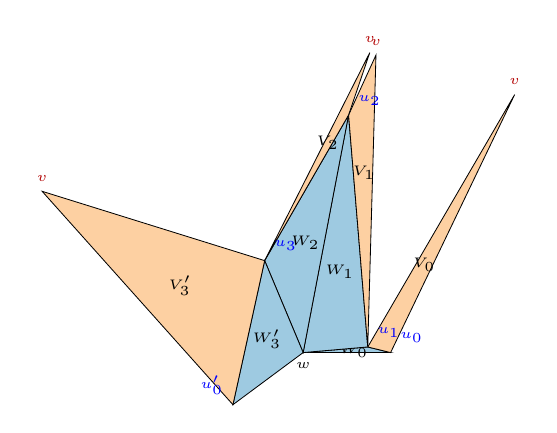
\begin{tikzpicture}[scale=0.3757, every node/.style={font=\tiny}]
  \draw[fill=fanblue, draw=black, line width=0.3pt] (0.0000,0.0000) -- (2.9560,0.0000) -- (2.1833,0.1897) -- cycle;
  \node at (1.7131,0.0632) {$W_{0}$};
  \draw[fill=petalorange, draw=black, line width=0.3pt] (7.1486,8.7204) -- (2.1833,0.1897) -- (2.9560,0.0000) -- cycle;
  \node at (4.0960,2.9701) {$V_{0}$};
  \draw[fill=fanblue, draw=black, line width=0.3pt] (0.0000,0.0000) -- (2.1833,0.1897) -- (1.5349,8.0305) -- cycle;
  \node at (1.2394,2.7401) {$W_{1}$};
  \draw[fill=petalorange, draw=black, line width=0.3pt] (2.4607,10.0564) -- (1.5349,8.0305) -- (2.1833,0.1897) -- cycle;
  \node at (2.0596,6.0922) {$V_{1}$};
  \draw[fill=fanblue, draw=black, line width=0.3pt] (0.0000,0.0000) -- (1.5349,8.0305) -- (-1.3019,3.1083) -- cycle;
  \node at (0.0777,3.7129) {$W_{2}$};
  \draw[fill=petalorange, draw=black, line width=0.3pt] (2.2520,10.1393) -- (-1.3019,3.1083) -- (1.5349,8.0305) -- cycle;
  \node at (0.8283,7.0927) {$V_{2}$};
  \draw[fill=fanblue, draw=black, line width=0.3pt] (-0.0000,0.0000) -- (-1.3019,3.1083) -- (-2.3738,-1.7615) -- cycle;
  \node at (-1.2252,0.4489) {$W_{3}'$};
  \draw[fill=petalorange, draw=black, line width=0.3pt] (-8.8236,5.4514) -- (-2.3738,-1.7615) -- (-1.3019,3.1083) -- cycle;
  \node at (-4.1664,2.2661) {$V_{3}'$};
  \node[blue, anchor=south west] at (2.9560,0.0000) {$u_{0}$};
  \node[red!70!black, anchor=south] at (7.1486,8.7204) {$v$};
  \node[blue, anchor=south west] at (2.1833,0.1897) {$u_{1}$};
  \node[red!70!black, anchor=south] at (2.4607,10.0564) {$v$};
  \node[blue, anchor=south west] at (1.5349,8.0305) {$u_{2}$};
  \node[red!70!black, anchor=south] at (2.2520,10.1393) {$v$};
  \node[blue, anchor=south west] at (-1.3019,3.1083) {$u_{3}$};
  \node[red!70!black, anchor=south] at (-8.8236,5.4514) {$v$};
  \node[blue, anchor=south east] at (-2.3738,-1.7615) {$u_0'$};
  \fill (0,0) circle (0.6pt) node[anchor=north] {$w$};

\end{tikzpicture}
\caption{A typical net $Z_k$ (fan faces blue, petals orange), $v$ the sharpest vertex, slit at the sharpest
neighbour $u_0$ of $w$.}
\end{figure}

\paragraph{Elementary consequences of (H).}
Since $\sum_x\kappa_x=4\pi$ over six vertices, (H) gives $\kappa_v\ge 2\pi/3$, hence
$\sum_i\nu_i=2\pi-\kappa_v\le 4\pi/3$. At any convex vertex each face angle is at most the sum of the other
face angles (the spherical polygon inequality for the tangent cone), so $\nu_j\le\frac12\sum_i\nu_i$, i.e.
\begin{equation}\label{numax}
 \nu_j\ \le\ \pi-\tfrac12\kappa_v\ \le\ \tfrac{2\pi}{3}\qquad\text{for every } j .
\end{equation}

\section{Reduction to three consecutive petals}

\begin{lemma}[petals do not cross interior hinges]\label{hinge}
In $Z_k$ no petal meets the relative interior of a hinge segment $wu_j$, $j\ne k$.
\end{lemma}
\begin{proof}
The two fan faces adjacent to $wu_j$ are $W_{j-1}$ and $W_j$; a petal crossing the segment would enter both.
Every petal shares a net vertex with $W_{j-1}$ or $W_j$ ($V_{j-1},V_j$ share $u_j$; $V_{j+1}$ shares $u_{j+1}$
with $W_j$; $V_{j-2}$ shares $u_{j-1}$ with $W_{j-1}$), and faces sharing a net vertex lie in disjoint
wedges there.
\end{proof}

\begin{lemma}[petal versus far fan face]\label{farfan}
If a petal $V_i$ overlaps a fan face $W_j$ with $j\notin\{i-1,i,i+1\}$ then $V_i$ overlaps $V_j$.
\end{lemma}
\begin{proof}
$V_i$ contains no vertex of $W_j$ ($w$ and the equator vertices of $W_j$ lie in fan faces or petals that share
a vertex with $V_i$, except possibly the local face $W_{k-1}'$, whose treatment is part of Lemma L).
By Lemma~\ref{hinge} the boundary of $V_i$ cannot enter $W_j$ through its hinges, so it enters through the
outer edge $u_ju_{j+1}$, which is the common edge of $W_j$ and $V_j$; near that crossing $V_i$ meets $V_j$.
\end{proof}

Hence Lemma F follows from the following statement about three consecutive petals, applied to the triples
$(V_k,V_{k+1},V_{k+2})$ and $(V_{k+1},V_{k+2},V_{k-1}')$ of $Z_k$.

\begin{conjecture}[Triple Lemma]\label{triple}
Let $W_i,W_j,W_{j+1}$ ($j=i+1$) be three consecutive fan faces of a net and $V_i,V_j,V_{j+1}$ their petals.
Under (H), $V_i$ and $V_{j+1}$ do not overlap.
\end{conjecture}

\begin{numerics}
No overlap of opposite petals under (H) in $72{,}000$ random nets, nor under the weaker hypothesis
$\kappa_v\ge\max\kappa_{u}$; adversarial hill-climbing (edges $\ge 0.05\,\mathrm{diam}$, curvatures $\ge 0.05$)
brings the two petals to within $0.4\%$ of the diameter but never into overlap. All observed overlaps
(44 in $72{,}000$ nets, without hypothesis) have two equator vertices sharper than $v$.
\end{numerics}

\section{Where a meeting can be}\label{sec:D}

Fix a triple as in Conjecture~\ref{triple} and write $u=u_j$, $u'=u_{j+1}$ for the base of $V_j$,
$\phi,\psi$ for the base angles of $V_j$ at $u,u'$, $\kappa=\kappa_u+\kappa_{u'}$.
In the net, $V_i$ and $V_j$ meet at $u$ only, separated there by the angular gap $\kappa_u$ between the two
copies $uv_j$ and $uv_i$ of the cut edge $uv$; likewise at $u'$.
Let $L$ be the line through $uv_i$ and $L'$ the line through $u'v_{j+1}$.

\begin{lemma}[double-outward wedge]\label{D}
$V_i$ lies in the closed half-plane of $L$ not containing $V_j$, and $V_{j+1}$ in the closed half-plane of
$L'$ not containing $V_j$. Hence every common point of $V_i$ and $V_{j+1}$ lies in
$\D:=$ the intersection of these two half-planes, which is the wedge at the point $p^*=L\cap L'$ opposite
to the base $uu'$. If $\kappa<\nu_j$ then $\D$ lies on $v_j$'s side of the base line (above), and if
$\kappa>\nu_j$ it lies on $w$'s side (below); $\D=\emptyset$ if $\kappa=\nu_j$.
\end{lemma}
\begin{proof}
The rays $uv_i$ and $u'v_{j+1}$ make angles $\phi+\kappa_u$ and $\psi+\kappa_{u'}$ with the base, so they
converge above the base iff $\phi+\psi+\kappa<\pi$, i.e. $\kappa<\nu_j$; the rest is the description of the
four wedges at $p^*$.
\end{proof}

\begin{lemma}[the two cut edges never cross]\label{nocross}
The segments $uv_i$ and $u'v_{j+1}$ are disjoint.
\end{lemma}
\begin{proof}
If they crossed at $p$ then $p$ would be above the base with base angles larger than $\phi,\psi$, so $v_j$
lies inside the triangle $uu'p$ and $|up|+|u'p|>|uv_j|+|u'v_j|=|uv_i|+|u'v_{j+1}|$, contradicting
$|up|\le|uv_i|$, $|u'p|\le|u'v_{j+1}|$.
\end{proof}

\begin{claim}[observed overlaps]
In the 44 observed opposite-petal overlaps (no hypothesis), the intersection region lies in $\D$; 26 are above
the base and 18 below, exactly as predicted by the sign of $\nu_j-\kappa$. In every below-base case the outer
edges $uu_i$ and $u'u_{j+2}$ of $W_i,W_{j+1}$ converge on $w$'s side (equivalently
$\angle_u W_i+\angle_u W_j+\angle_{u'}W_j+\angle_{u'}W_{j+1}<\pi$) and exactly one of the two fan faces
extends past the crossing point; both cannot, since fan faces are disjoint.
\end{claim}

\begin{figure}[h]\centering
% Labels offset by hand for this very thin numerical example.
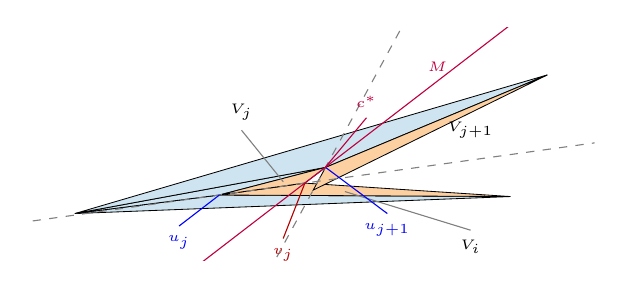
\begin{tikzpicture}[scale=0.2645, every node/.style={font=\tiny}]
  \clip (-2.2683,-2.2683) rectangle (24.9509,8.9249);
  \draw[fill=fanblue!50, draw=black, line width=0.3pt] (0.0000,0.0000) -- (20.9062,0.8161) -- (6.9374,0.8902) -- cycle;

  \draw[fill=fanblue!50, draw=black, line width=0.3pt] (0.0000,0.0000) -- (6.9374,0.8902) -- (12.0354,2.2168) -- cycle;

  \draw[fill=fanblue!50, draw=black, line width=0.3pt] (0.0000,0.0000) -- (12.0354,2.2168) -- (22.6826,6.6566) -- cycle;

  \draw[fill=petalorange, draw=black, line width=0.3pt] (11.0451,1.4611) -- (6.9374,0.8902) -- (20.9062,0.8161) -- cycle;
  \draw[gray,thin] (12.9629,1.0558) -- (19,-0.8) node[black,anchor=north] {$V_i$};
  \draw[fill=petalorange, draw=black, line width=0.3pt] (11.0443,1.4667) -- (12.0354,2.2168) -- (6.9374,0.8902) -- cycle;
  \draw[gray,thin] (10.0057,1.5246) -- (8,4) node[black,anchor=south] {$V_j$};
  \draw[fill=petalorange, draw=black, line width=0.3pt] (11.4415,1.1249) -- (22.6826,6.6566) -- (12.0354,2.2168) -- cycle;
  \node at (19,4) {$V_{j+1}$};
  \draw[dashed, gray] (-60.4627,-8.4762) -- (74.3374,10.2566);
  \draw[dashed, gray] (44.5479,61.9951) -- (-20.4771,-57.5614);
  \draw[blue,thin] (6.9374,0.8902) -- (5,-0.6) node[anchor=north] {$u_j$};
  \draw[blue,thin] (12.0354,2.2168) -- (15,0) node[anchor=north] {$u_{j+1}$};
  \draw[red!70!black,thin] (11.0443,1.4667) -- (10,-1.2) node[anchor=north] {$v_j$};
  \fill[purple] (12.0185,2.2161) circle (0.8pt);
  \draw[purple,thin] (12.0185,2.2161) -- (14,4.6) node[anchor=south] {$c^*$};
  \draw[purple, thin] (22.8053,10.5147) -- (-20.3417,-22.6795) node[pos=0.125,anchor=south] {$M$};
\end{tikzpicture}

\caption{An above-base overlap (no hypothesis): the region $\D$ beyond $p^*$, the point $c^*$ and the line $M$
of \S\ref{sec:cstar}. Here $\nu_i+\nu_j>\pi$ and $V_i$ crosses $M$.}
\end{figure}

\section{The rotation picture (above-base case)}\label{sec:cstar}

Glue $V_i,V_j,V_{j+1}$ flat around $v$ with no gaps (the ``$v$-fan''); this is possible because
$\nu_i+\nu_j+\nu_{j+1}<2\pi$, and in it the three petals occupy disjoint wedges at $v$. The net position of
$V_i$ is obtained from its $v$-fan position by the rotation $\rho_u$ about $u$ by the gap angle $\kappa_u$
(away from $V_j$), and that of $V_{j+1}$ by the rotation $\rho_{u'}$ about $u'$ by $\kappa_{u'}$. Both
rotations have the same sense. Therefore
\[
 V_i\cap V_{j+1}\neq\emptyset\ \text{ in the net }\iff\ \R(V_i^{\rm fan})\cap V_{j+1}^{\rm fan}\neq\emptyset,
 \qquad \R:=\rho_{u'}^{-1}\circ\rho_u,
\]
and $\R$ is the rotation by $\kappa=\kappa_u+\kappa_{u'}$ about the point $c^*$ on $w$'s side of the base
with $\angle c^*uu'=\kappa_u/2$, $\angle uu'c^*=\kappa_{u'}/2$ (composition of two rotations).
Let $M$ be the line $c^*v$; $\R$ moves points from $u'$'s side of $M$ towards $u$'s side. Measure angles
around $c^*$ from $M$, positively towards $u$'s side.

\begin{lemma}[angular criterion]\label{angular}
Let $\varepsilon_i\ge0$ be the largest angle (seen from $c^*$) by which $V_i^{\rm fan}\cap\{\text{above the base}\}$
crosses $M$ towards $u'$'s side, and $\varepsilon_{j+1}$ the corresponding excursion of
$V_{j+1}^{\rm fan}\cap\{\text{above}\}$ towards $u$'s side. If $\kappa<\nu_j$ and
\begin{equation}\label{epscrit}
 \varepsilon_i+\varepsilon_{j+1}\ <\ \kappa ,
\end{equation}
then $V_i$ and $V_{j+1}$ do not overlap in the net.
\end{lemma}
\begin{proof}
By Lemma~\ref{D} a common point $p$ is above the base. The rotation $\rho_u^{-1}$ maps the wedge of $V_i$ at
$u$ in the net, $[\phi+\kappa_u,\ 2\pi-\angle_uW_j-\angle_uW_i]$, onto the $v$-fan wedge, so $x=\rho_u^{-1}(p)$
is below the base only if $p$ is; hence $x\in V_i^{\rm fan}$ and $y=\rho_{u'}(p)\in V_{j+1}^{\rm fan}$ are above the
base and $y=\R(x)$. Their angles from $M$ satisfy $\theta_y=\theta_x+\kappa$ with
$\theta_x\ge-\varepsilon_i$ and $\theta_y\le\varepsilon_{j+1}$, so $\kappa\le\varepsilon_i+\varepsilon_{j+1}$
(no wrap-around since $\kappa<\nu_j<\pi$).
\end{proof}

In particular, if neither petal crosses $M$ above the base ($\varepsilon_i=\varepsilon_{j+1}=0$), there is no
overlap. When does a petal cross $M$? Write $\mu_u=\angle uvc^*$, $\mu_{u'}=\angle c^*vu'$, so
$\mu_u+\mu_{u'}=\nu_j$ ($c^*$ lies in the cone of $V_j$ at $v$, being on $w$'s side of the base between the
lines $vu$, $vu'$). The wedge of $V_i$ at $v$ starts at $vu$ and turns away from $V_j$ by $\nu_i$; it reaches
the ray of $M$ beyond $v$ iff $\nu_i>\pi-\mu_u$. The other way for $V_i^{\rm fan}\cap\{\text{above}\}$ to cross $M$
is through the far vertex $u_i$ or through the point where the edge $vu_i$ or $uu_i$ crosses the base line.

\begin{lemma}\label{notboth}
Under (H) the two petals cannot both cross $M$ through their wedges at $v$.
\end{lemma}
\begin{proof}
That would need $\nu_i+\mu_u>\pi$ and $\nu_{j+1}+\mu_{u'}>\pi$, hence $\nu_i+\nu_{j+1}+\nu_j>2\pi$, whereas
$\nu_i+\nu_j+\nu_{j+1}\le\sum\nu\le 4\pi/3$.
\end{proof}

\begin{lemma}[the above-base case needs a very sharp $v$]\label{sharp}
Under (H), $\kappa<\nu_j$ forces $\kappa_v>6\pi/7$, hence $\sum_i\nu_i<8\pi/7$ and each $\nu_i<4\pi/7$.
\end{lemma}
\begin{proof}
$4\pi=\sum_x\kappa_x\le 4\kappa_v+\kappa$ and $\kappa<\nu_j\le\pi-\kappa_v/2$ by \eqref{numax}.
\end{proof}

\begin{numerics}
In $3000$ random octahedra (all apexes, all triples with $\kappa<\nu_j$): the composition $\R$ has the stated
centre and sense, and the criterion of Lemma~\ref{angular} reproduces the net overlap test exactly.
Under (H) neither petal ever crosses $M$ above the base ($\varepsilon_i=\varepsilon_{j+1}=0$ in all $224$
triples, degenerate ones included), and adversarial search under (H) cannot make either excursion positive.
Under the weaker hypothesis $\kappa_v\ge\max\kappa_u$ a petal can cross $M$ and \eqref{epscrit} can fail
(excursion $1.96$ with $\kappa=0.05$), so (H) is genuinely used. Every one of the 26 observed above-base
overlaps violates $\varepsilon_i=\varepsilon_{j+1}=0$ (20 through $V_i$, 6 through $V_{j+1}$).
\end{numerics}

\begin{figure}[h]\centering
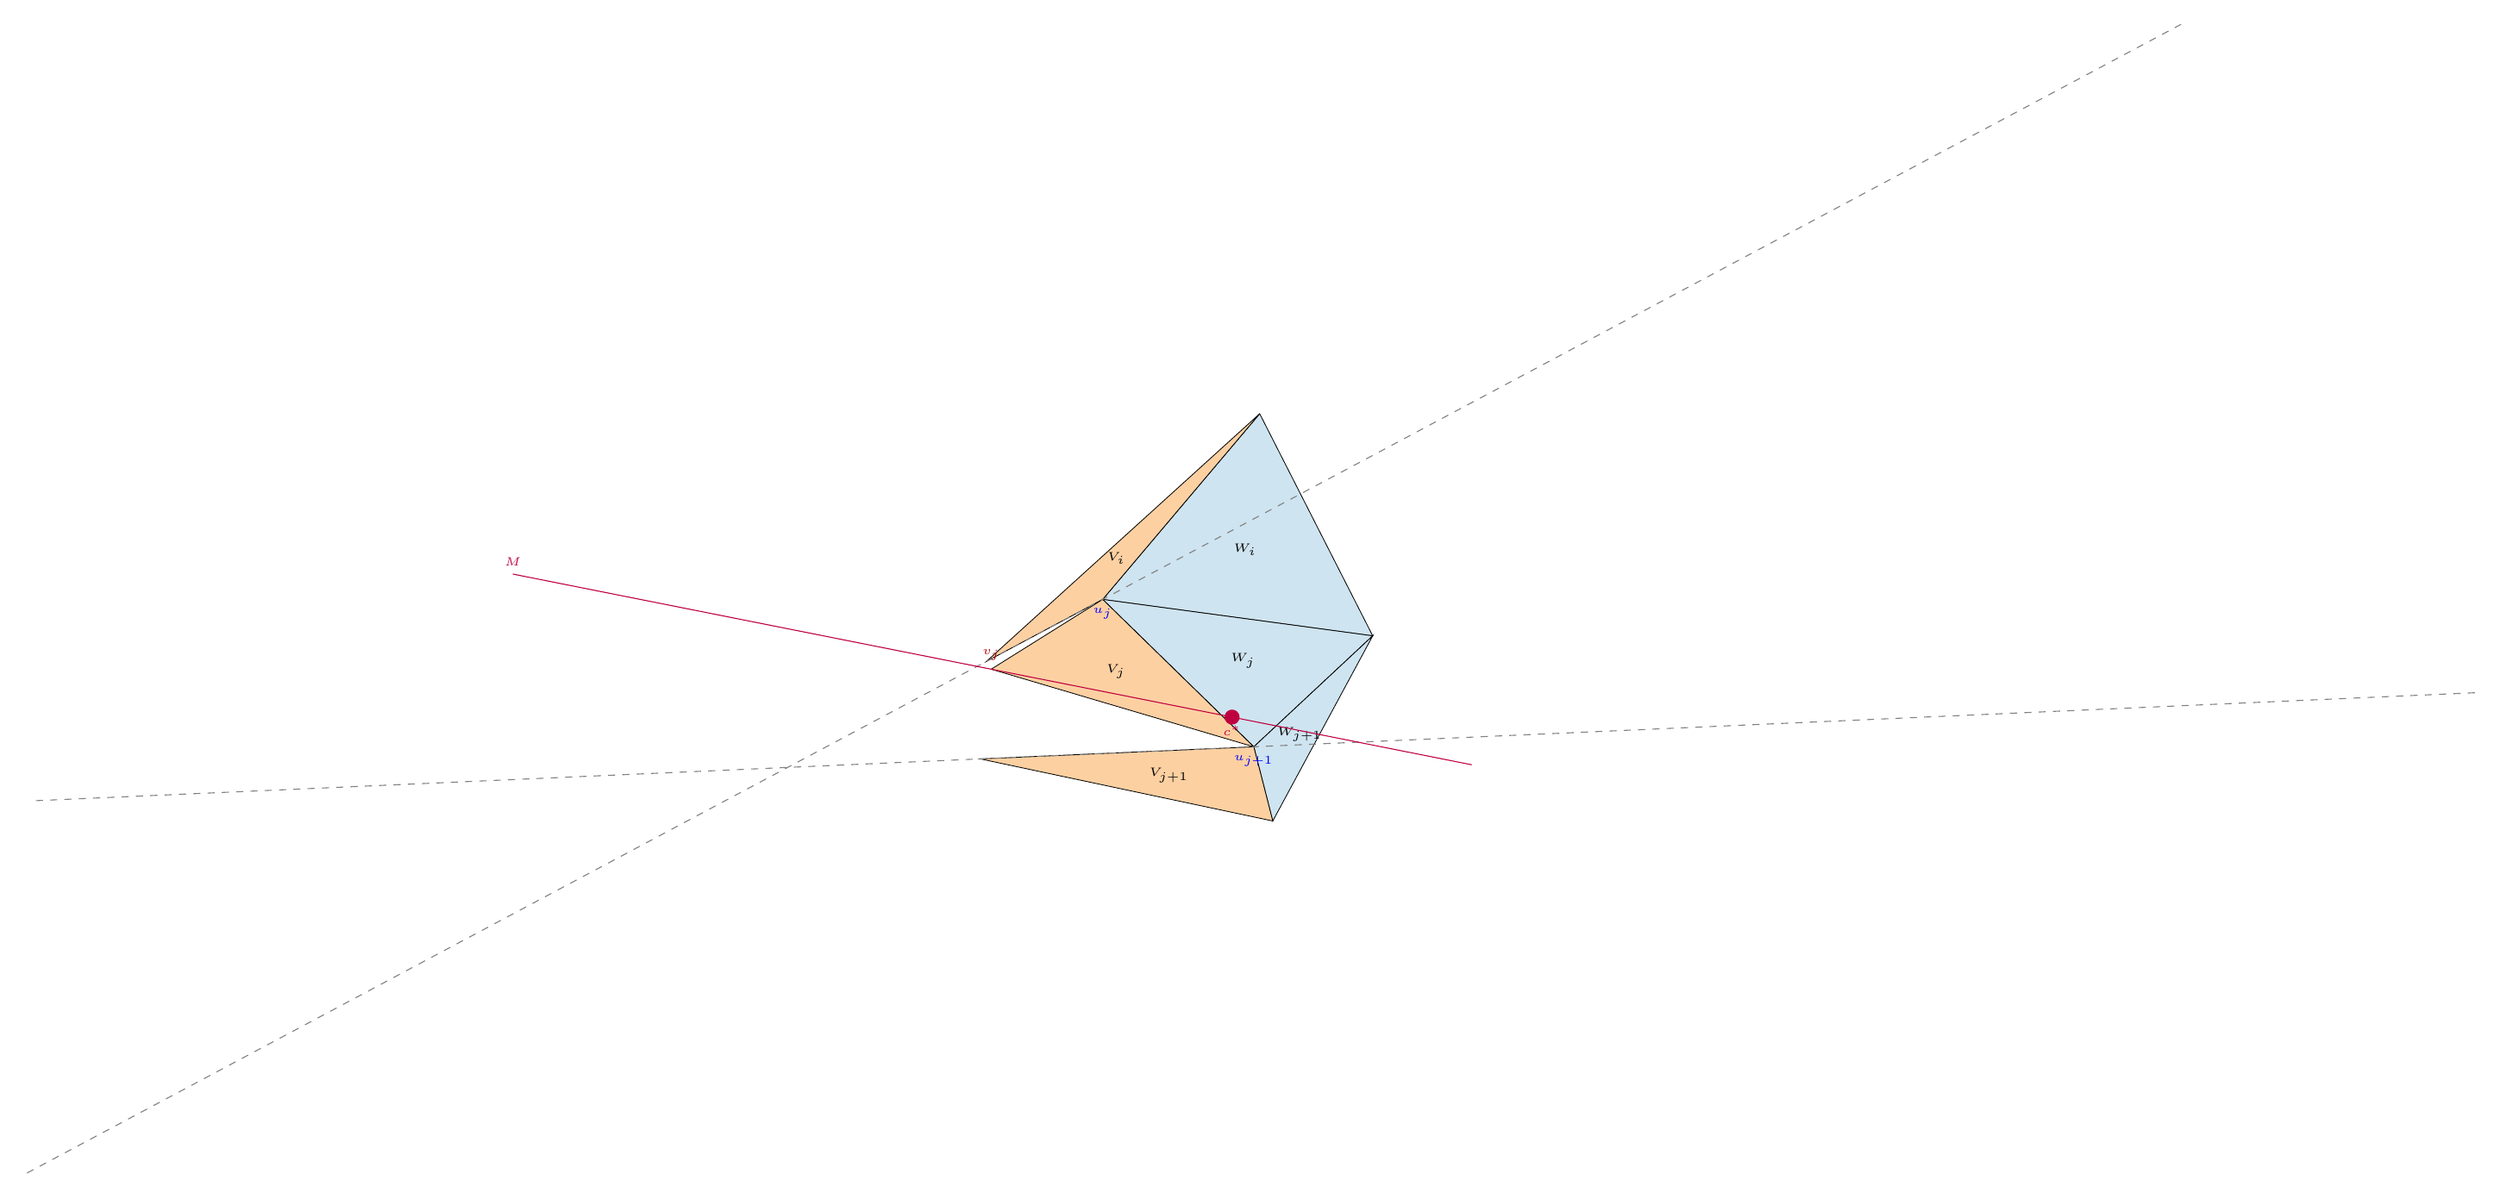
\begin{tikzpicture}[scale=3.9352, every node/.style={font=\tiny}]
  \draw[fill=fanblue!50, draw=black, line width=0.3pt] (-0.0000,0.0000) -- (-0.4230,0.8315) -- (-1.0105,0.1364) -- cycle;
  \node at (-0.4778,0.3226) {$W_i$};
  \draw[fill=fanblue!50, draw=black, line width=0.3pt] (-0.0000,0.0000) -- (-1.0105,0.1364) -- (-0.4450,-0.4155) -- cycle;
  \node at (-0.4852,-0.0930) {$W_j$};
  \draw[fill=fanblue!50, draw=black, line width=0.3pt] (0.0000,-0.0000) -- (-0.4450,-0.4155) -- (-0.3740,-0.6932) -- cycle;
  \node at (-0.2730,-0.3695) {$W_{j+1}$};
  \draw[fill=petalorange, draw=black, line width=0.3pt] (-1.4448,-0.0953) -- (-1.0105,0.1364) -- (-0.4230,0.8315) -- cycle;
  \node at (-0.9594,0.2909) {$V_i$};
  \draw[fill=petalorange, draw=black, line width=0.3pt] (-1.4277,-0.1249) -- (-0.4450,-0.4155) -- (-1.0105,0.1364) -- cycle;
  \node at (-0.9611,-0.1347) {$V_j$};
  \draw[fill=petalorange, draw=black, line width=0.3pt] (-1.4687,-0.4608) -- (-0.3740,-0.6932) -- (-0.4450,-0.4155) -- cycle;
  \node at (-0.7626,-0.5232) {$V_{j+1}$};
  \draw[dashed, gray] (3.0252,2.2895) -- (-5.0461,-2.0167);
  \draw[dashed, gray] (4.1246,-0.2131) -- (-5.0147,-0.6178);
  \node[blue, anchor=north] at (-1.0105,0.1364) {$u_j$};  \node[blue, anchor=north] at (-0.4450,-0.4155) {$u_{j+1}$};
  \node[red!70!black, anchor=south] at (-1.4277,-0.1249) {$v_j$};
  \fill[purple] (-0.5264,-0.3043) circle (0.8pt) node[anchor=north] {$c^*$};
  \draw[purple, thin] (0.3708,-0.4828) -- (-3.2181,0.2313) node[anchor=south] {$M$};
\end{tikzpicture}
\caption{A triple under (H) with $\kappa<\nu_j$: $c^*$, the line $M$ and the two dashed cut-edge lines; both
petals stay on their own side of $M$.}
\end{figure}

\paragraph{What remains for the above-base case.}
Prove that under (H) and $\kappa<\nu_j$ neither $V_i^{\rm fan}\cap\{\text{above}\}$ nor
$V_{j+1}^{\rm fan}\cap\{\text{above}\}$ crosses $M$ (or, more weakly, that \eqref{epscrit} holds). The three
crossing mechanisms are: (a) the wedge at $v$: $\nu_i>\pi-\mu_u$; (b) the far vertex $u_i$ above the base on
$u'$'s side of $M$; (c) an edge of $V_i$ crossing the base line outside the segment $uu'$ on $u'$'s side of $M$.
Mechanism (c) through $vu_i$ requires $\nu_i+\nu_j>\pi+\psi$; (a) requires $\nu_i+\nu_j>\pi$; by
Lemma~\ref{sharp} these need $\kappa_v<\pi$ and two of the four angles at $v$ close to $4\pi/7$. The numerics
say the fan faces then obstruct this, but the argument is not yet written.

\section{The below-base case}

When $\kappa>\nu_j$ the wedge $\D$ lies on $w$'s side of the base. Then (Claim above) a meeting requires the
outer-edge lines of $W_i$ and $W_{j+1}$ to converge on $w$'s side, one of the two fan faces to reach past
their crossing point $X$, and the opposite petal to pass over the far vertex of that fan face. In the observed
below-base overlaps two equator vertices have curvature close to $2\pi$ and $v$ is nearly flat. Under (H),
$\kappa_u,\kappa_{u'}\le\kappa_v$ and $\nu_j<\kappa\le 2\kappa_v$; no proof yet.

\section{Known false / do not retry}
Simple separating lines for the two petals inside $\D$ (bisector of $\D$ at $p^*$, lines through $v_j$) fail
in about a third of the non-degenerate cases even under (H): the separation is a rotation phenomenon, not a
half-plane one. The six wedge--lean inequalities of the handoff fail in $0.5\%$ of nets under (H) (needle-like
$w$), so they cannot replace the argument above.

\section*{Code}
\texttt{octa.py} (module: all quantities, nets $Z_k$, nine pairs, intersection polygons),
\texttt{vwedge.py}, \texttt{oppcases.py} (collect/classify/draw overlaps), \texttt{adv\_opp.py} (adversarial
separation), \texttt{cstar.py} (checks of \S\ref{sec:cstar}), \texttt{adv\_eps.py}, \texttt{adv\_mu.py},
\texttt{adv\_cstar.py} (adversarial tests of \eqref{epscrit} and of the crossing conditions),
\texttt{tikz\_net.py} (figures), \texttt{draw.py} (PNG).
\end{document}
